\documentclass[12pt]{article}
\usepackage[utf8]{inputenc}
\usepackage{geometry}
\usepackage{graphicx}
\usepackage{hyperref}
\usepackage{amsmath}
\usepackage{caption}
\usepackage{enumitem}
\geometry{margin=1in}

% Title information
\title{Project Proposal: RISC-V Processor Implementation with DSP Support}
\author{Group: Jonathan Warner, Giovanni Gutierrez, Jaron Tsao, Jacob Jelovich}
\date{ECE 6710 \\ Dr. P.-E. Gaillardon \\ \today }

\begin{document}

\begin{flushleft}
    {ECE 6710 \\ Dr. P.-E. Gaillardon \\ \today} \\[2em]
\end{flushleft}
\begin{center}
    \textbf{Project Proposal: RISC-V Processor Implementation with DSP Support} \\[2em]
\end{center}

\begin{flushleft}
    {Group: Jonathan Warner, Giovanni Gutierrez, Jaron Tsao, Jacob Jelovich}
\end{flushleft}
\hrule
\vspace{1em}

\section*{Motivation}
To achieve high performance for a generalized processor that allows for DSP implementation.  This eliminates the need for external DSP chips and can allow for custom and efficient computing for DSP workloads.

\section*{High Level Description}
The goal of our project is to develop a fully functional RISC-V processor with extensions and hardware support for Discrete Signal Processing.

\subsection*{Stretch Goals}

\begin{itemize}
    \item Branch prediction
    \item Pipelined execution
    \item Dynamic scheduling
    \item FPU using Takum arithmetic \cite{hunhold2024beatingpositsgametakum}
\end{itemize}

\section*{Functional Block Diagram}
We will use an architecture suited for DSP use with a 4 or 5-stage pipeline, similar to the one shown below. We may include different outputs and data memory to make our design more general, but this diagram is suitable to show the big ideas behind what we will be doing.

\begin{figure}[h!]
    \centering
    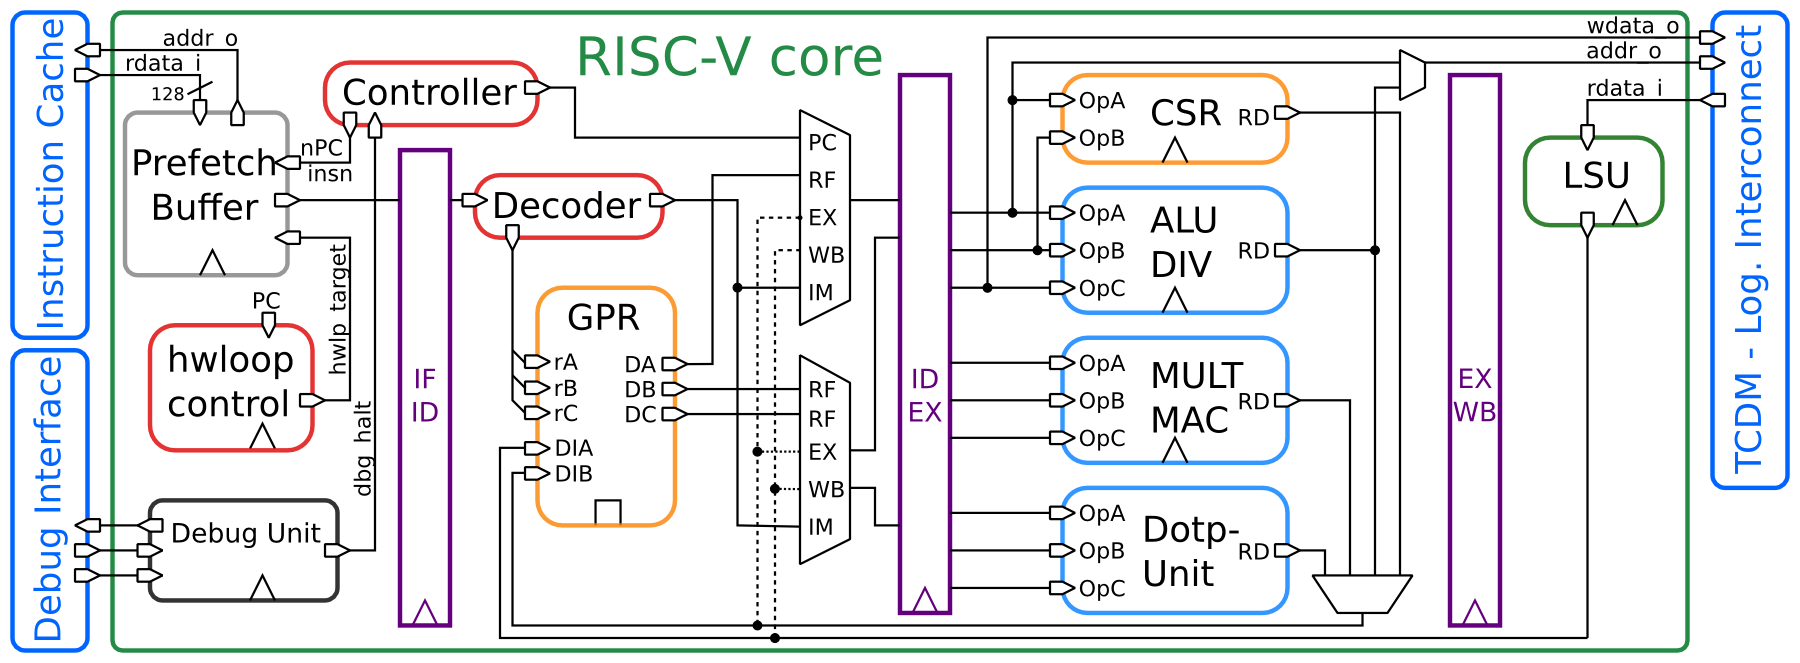
\includegraphics[width=\linewidth]{Proposal/core_archi.png}
    \caption{RISC-V Pipeline Architecture for a 4-stage Pipeline with DSP and TCDM Support \cite{gautschi2016nearthresholdriscvcoredsp}}
    \label{fig:block-diagram}
\end{figure}

\section*{Testing Options}
Using a custom linker script and the right version of GCC, we can write and compile a comprehensive C program to upload to memory on an FPGA board to test our design. If we were to fabricate the chip, we would want to design a different memory controller to interface with external memory rather than using RAM on an FPGA. Otherwise, we can effectively test integration of our complete system in this way. The testing process is as follows:

\begin{enumerate}
    \item Ensure that each hardware module works as intended using testbenches and ModelSim simulations
    \item Write a comprehensive program to test system integration using an FPGA board
    \item Simulate the mapped netlist after logic synthesis to understand circuit performance and area
    \item Run post physical synthesis (P\&R) simulations before fabrication to verify proper functionality
\end{enumerate}

% TODO summary of required external signals and I/O interface for simulation

\section*{Roles}

\begin{itemize}
    \item ALU and FPU modules: Jonathan and Jacob
    \item DSP module(s): Giovanni and Jaron
    \item Memory and I/O controller(s): Everyone
    \item System integration: Jonathan and Jacob
    \item Programming: TBD
\end{itemize}

\bibliographystyle{IEEEtran}
\bibliography{references}

\end{document}
